\newpage
\section{Related Work}
\label{sec:relatedWork}

\iffalse
\hl{Contents:}
\begin{itemize}
\item \hl{A survey of the literature (journals, conferences, book chapters) on the areas that are relevant to your research question. One section per area.
The chapter should conclude with a summary of the previous research results that you want to develop further or challenge. The summary could be presented in a model, a list of issues, etc. Each issue could be a chapter in the presentation of results. They should definitely be discussed in the discussion / conclusion of the thesis.}
\item \hl{The Literature Review provides the necessary background information to familiarize the reader with prior research and relevant theory.  Three general types of literature reviews exist:  the broad scan, the focused review, and the comprehensive critique.}
\end{itemize}

\begin{itemize}
\item \hl{More than a literature review}
\item \hl{Organize related work - impose structure}
\item \hl{Be clear as to how previous work being described relates to your own.}
\item \hl{The reader should not be left wondering why you've described something!!}
\item \hl{Critique the existing work - Where is it strong where is it weak? What are the unreasonable/undesirable assumptions?}
\item \hl{Identify opportunities for more research (i.e., your thesis) Are there unaddressed, or more important related topics?}
\item \hl{After reading this chapter, one should understand the motivation for and importance of your thesis}
\item \hl{You should clearly and precisely define all of the key concepts dealt with in the rest of the thesis, and teach the reader what s/he needs to know to understand the rest of the thesis.}
\end{itemize}
\fi

% Matrix Factorization
%First mentioned: Yannakakis 1990
% In machine learning: Lee, Seung 1999
%https://www.youtube.com/watch?v=kSfwY68gQ9I

\subsection{Role Mining with Data Mining}
\hl{SECTION UNDER CONSTRUCTION}\\
Role Mining has been first coined in \cite{Kuhlmann}. In the following years several researchers have analyzed Role Mining further and defined several Role Mining Problems, Quality Measures, Cleaning Techniques and Algorithms.
\subsection{Role Mining of "Meaningful Roles"}
\label{sec:meaningfulRoles}
\hl{SECTION UNDER CONSTRUCTION}\\
In the recent years several researchers are investigating the problem finding "meaningful" roles, since the classic Role Mining approaches outputs RBAC models, which are often not accepted in practice.\\
\cite{Xu}
\subsection{Role Mining with Bio-inspired Techniques}
\hl{SECTION UNDER CONSTRUCTION}\\
In \cite{Igor} and \cite{saenko2012design} the Basic RMP and the Min-Edge RMP are tackled with a genetic algorithm (GA). For the evaluation function of the GA the authors combine several objectives in one single objective maximization function, where the fitness values for each objective are weighted. The objectives for the Basic RMP are the minimization of roles, confidentiality violations and availability violations. A confidentiality violation expresses a situation where a user would get an access right due to the generated role model, which he or she did not had in the current access control configuration. An availability violation on the other hand expresses if a user gets an access right less than he or she did had in the current access control configuration. For the Min-Edge RMP the objective of minimizing roles is exchanged with minimizing the number of user-role- and role-permission assignments.\\
In a first version of the approach the authors choose a representation of role models as individuals consisting of three chromosomes: A chromosome $X$, which represents the UA-Matrix, a chromosome $Y$, which represents the PA-Matrix, and a control-chromosome $Z$, which controls if a role is active or passive. With the control-chromosome they influence how many roles a role model has and make it possible to vary the amount with variation operators of the GA. The authors suggest a crossover function in three phases, which is particularly designed for the suggested multi-chromosomal representation. The drawback of this approach are unnecessary passive genes. The chromosomes X and Y, respectively the UA- and PA-Matrix, contain roles, which are passive (controlled by chromosome Z).\\
Due to this drawback the authors came up with an improved representation where they combine the X and Y chromosome into one variable-length chromosome and get rid of the control-chromosome Z. A role model is now representation as chromosome where a gene represents a role. A gene (role) consists of a user-list ($L_X$) and a permission-list ($L_Y$). Due to the change of representation the crossover method is changed accordingly. As shown in figure \ref{fig:crossover} the author suggest to use a traditional one-point crossover, where the points of crossover of two individuals are randomly chosen. After the crossover operation a local optimization of offspring chromosomes is executed, where genes with same user-lists or permission-lists are combined.
\begin{figure}[H]
    \centering
    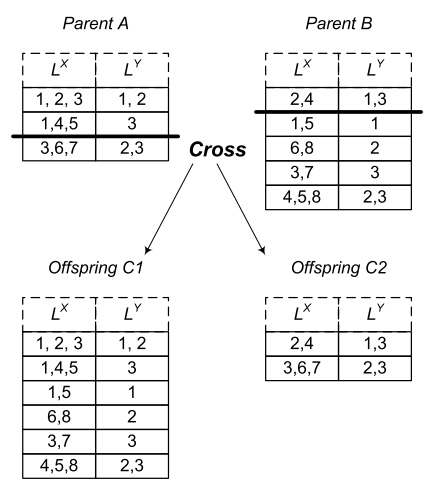
\includegraphics[scale=0.8]{./Figures/crossover.png}
    \rule{20em}{0.5pt}
    \caption{Examples of the crossover in the improved GA for the RMP by Saenko et al.\cite{saenko2012design}}
    \label{fig:crossover}
\end{figure}
The first approach is tested on randomly generated data with three different dimensions\cite{Igor}. The evaluation is on the number of generations needed to obtain a solution which meet the suggested evaluation function. The performance of the first and the improved GA are compared with the result that the improved GA has a better performance in all dimensions of UPA, especially in greater dimensions\cite{saenko2012design}. No further evaluations on the resulting role models in the suggested approaches are done. In the recent paper \cite{Kotenko:2015} the authors focusing on the multi-chromosomal approach again.\\
In this thesis the suggested improved approach is used as starting point in my approach to deal with the basic RMP.\\\\
In \cite{DuChang} the authors propose a genetic algorithm (GA)-based and an ant-colony-optimization (ACO)-based algorithm for the ideas in \cite{Xu} (see section \ref{sec:meaningfulRoles}), where a previously mined set of candidate roles is optimized. The focus is on the objectives of the basic RMP and on the interpretability of roles, where a role is considered meaningful if its assigned users can be characterized by an expression of user attributes. The goal is finding optimal candidate roles for an RBAC$_1$ role model (role model with role hierarchy).\\
In the GA-based algorithm a set of all candidate roles is reduced by repeatedly removing roles, while in the ACO-based algorithm it is started with an empty candidate role set, where roles are repeatedly added.

\iffalse
\\
elite strategy where the fittest individual of a generation is kept in the next generation

\\
Which data? publicly available access control policies
Comparison? proposed algorithms achieves better performance than the corresponding existing algorithms, GA-based approach produces better results than ACO-based approach.
\\\\
In \cite{paper} an evolutionary approach for solving the policy generation problem is introduced.
\fi